\chapter{Gangfræði}

Helsta markmið aflfræðinnar er að ákvarða staðsetningu hluta sem fall af tíma. Á síðari hluta 19. aldar á William Thomson (einnig þekktur sem Lord Kelvin) að hafa sagt að það væri ekkert eftir til þess að uppgötva í eðlisfræði lengur. Það eina sem eðlisfræðingar ættu eftir ógert væri að reikna fleiri aukastafi með betri mælitækjum og nálgunum. Honum skjátlaðist sem betur fer hrapalega!

\section{Staða, hraði og hröðun}

Við skulum byrja á því að tala um einvíða hreyfingu. Það er mikilvægt að nefna að það er alltaf hægt að snúa hnitakerfinu þannig að hreyfing hlutarins sé aðeins í eina vídd. 

\begin{tcolorbox}
\begin{definition}
    Lítum á hlut sem hreyfist í einni vídd. \textbf{Staðsetning} hlutarins er táknuð með $s$. Við skrifum stundum $s(t)$ til þess að taka fram að staðsetningin $s$ sé fall af tíma, $t$. Við notum iðulega ritháttinn $s_0$ til þess að tákna \textbf{upphafsstaðsetningu} hlutarins. \textbf{Færsla} hlutarins frá staðsetningu $s_1$ til $s_2$ er táknuð með $\Delta s = s_2 - s_1$. 
\end{definition}
\end{tcolorbox}
Takið eftir að upphafsstaðsetningin er miðuð við tímann þar sem við byrjum mælingu. Okkur er frjálst að stilla klukkurnar okkar þannig að hún sýnir upphafstímann sem $t_0 = 0$ þegar hluturinn er í upphafsstaðsetningu sinni. Það er mjög hentugt þar sem að við höfum einungis áhuga á breytingu í tíma, þ.e.a.s.~$\Delta t = t - t_0$, en þá með því að velja $t_0 = 0$ þá höfum við að $\Delta t = t$. \\

Okkur er því bæði frjálst að stilla klukkurnar okkar á $t = 0$ og að velja hnitakerfið okkar þannig að $s_0 = 0$.\\

Þegar við hugsum um orðið hraði, þá tengjum við það iðulega við upplifuna okkar af því í daglegu tali sem er oftast í tengslum við bíla og önnur farartæki, t.d~rafmagnshlaupahjólin frá Hopp. Við hugsum um það sem mælikvarða á það hversu fljót við erum á milli tveggja staða $s_a$ og $s_b$. Ef við keyrum hratt þá komumst við fljótt á staðinn! Það sem fólk gleymir að taka inn í reikninginn er að það skiptir líka gríðarlega miklu máli hvort að við séum að breyta hraðanum okkar á leiðinni. Við erum til dæmis mjög lengi að hlaupa maraþon ef við tökum okkur tveggja tíma lúr í miðju hlaupi. Breyting í hraða nefnist hröðun. Ef engin hröðun verkar á farartækið þá tölum við um að það ferðist með jöfnum hraða. Ef við keyrum með jöfnum hraða $\SI{90}{km/klst}$ þá er auðvelt að áætla hversu lengi við erum á leiðinni til Selfossar sem er í $\SI{60}{km}$ fjarlægð. Það er því eðlilegt að skilgreina (sérstaklega miðað við einingarnar)
\begin{tcolorbox}
\begin{definition}
Lítum á hlut sem ferðast frá upphafsstaðsetningu $s_0$ til $s_1$ á tíma $t$. \textbf{Meðalhraði} hlutarins, $v_m$, er þá skilgreindur þannig að:
\begin{align*}
    v_m := \frac{s_1 - s_0}{t} = \frac{\Delta s}{\Delta t}.
\end{align*}
\end{definition}
\end{tcolorbox}

Hinsvegar þá keyrum við ekki alltaf með jöfnum hraða. Því miður virkar umferðin ekki nema að sumir stoppi stundum á rauðu ljósi. Þess vegna er skilgreining að ofan ekkert sérlega góð. Til þess að betrumbæta hana þá getum við skoðað meðalhraðan á styttri tímabilum. Þegar tímabilið $\Delta t$ verður örlítið (og þar með líka vegalengdin $\Delta s$) þá fáum við það sem kallast augnablikshraði hlutarins, sem er það sem við köllum einfaldlega hraða hlutarins. Það er hraðinn sem þið sjáið í mælaborði bílsins. Til þess að útskýra þetta nánar skulum við kynna tvö afar hentug tól, þ.e.a.s.~stöðu-tíma grafið og hraða-tíma grafið.


\begin{figure}[H]
    \centering
\begin{subfigure}[h]{0.4\textwidth}
    \centering
    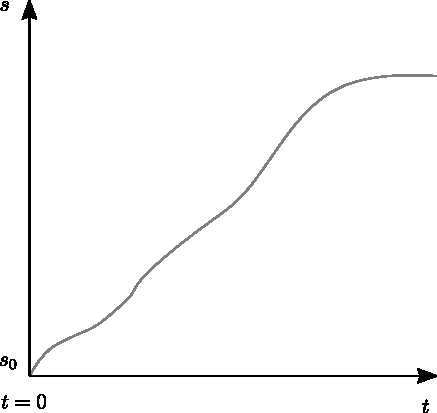
\includegraphics[width=\linewidth]{figures/stodutimagraf.pdf}
    \label{fig:stgraph}
\end{subfigure}
\hfill
\begin{subfigure}[h]{0.4\textwidth}
    \centering
    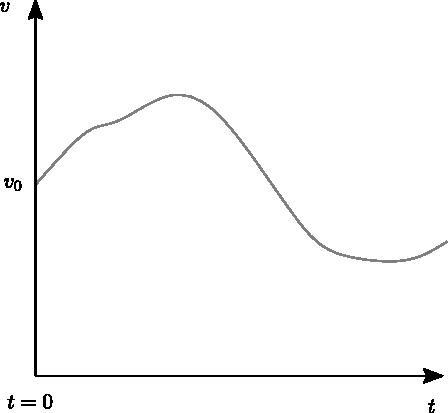
\includegraphics[width=\linewidth]{figures/hradatimagraf.pdf}
    \label{fig:vtgraph}
\end{subfigure}
\caption{Hér má sjá vinstra meginn stöðu sem fall af tíma og hægra meginn hraða sem fall af tíma.}
\end{figure}

Á stöðu-tíma grafinu þá teiknum við stöðu hlutar, $s$, sem fall af tíma $t$. Við teiknum það oft þannig að $s_0 = 0$ við $t = 0$ eins og sést á mynd \ref{fig:stgraph} hér að ofan. Á hraða-tíma grafinu þá teiknum við hraða hlutarins, $v$, sem fall af tíma $t$. Við getum hinsvegar ekki eins auðveldlega skilgreint upphafshraðann $v_0$ þannig að hann sé núll (það er samt hægt en þá þurfum við að tala um afstæða hreyfingu!). Dæmi um slíkt graf má sjá á mynd \ref{fig:vtgraph} hér að ofan. \\


\begin{figure}[H]
    \centering
\begin{subfigure}[h]{.4\textwidth}
    \centering
    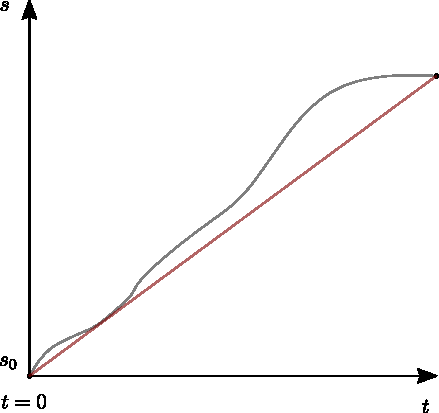
\includegraphics[width=\linewidth]{figures/stodutimagraf-medalhradi.pdf}
    \caption{Á þessu stöðu-tíma grafi táknar rauða línan feril hlutar sem hefði haft fastan meðalhraða.}
    \label{fig:st-medalhradi}
\end{subfigure}
\hfill
\begin{subfigure}[h]{.4\textwidth}
    \centering
    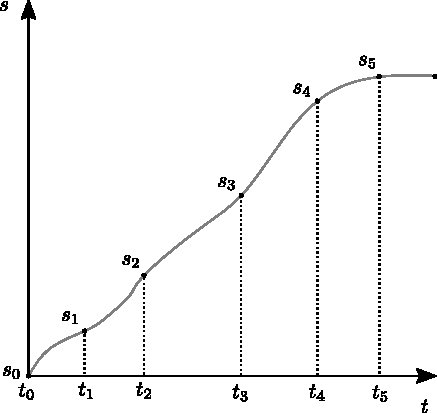
\includegraphics[width=\linewidth]{figures/stodutimagraf-skiptingar.pdf}
    \caption{Til að fá nákvæmara mat á hraðann þá er heildartíminn brotinn niður í minni tímabil.}
    \label{fig:st-skiptingar}
\end{subfigure}
\caption{Vinstra meginn sést munurinn á hlut sem ferðast með breytilegum hraða og hlut sem ferðast með föstum hraða. Hægra meginn sést sami ferill þar sem við bætt við skiptipunktum til að minnka tímabilið.}
\end{figure}

\begin{figure}[H]
    \centering
\begin{subfigure}[h]{.4\textwidth}
    \centering
    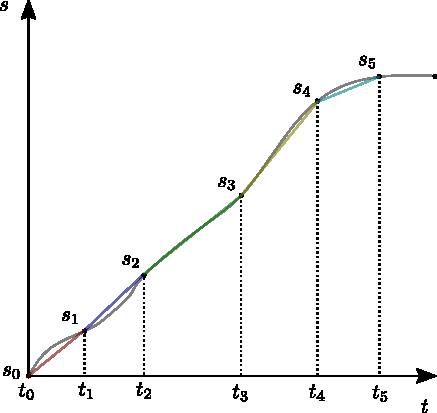
\includegraphics[width=\linewidth]{figures/stodutimagraf-skiptingar-linur.pdf}
    \caption{Því minni tímabil sem við veljum, því betra mat á raunverulegan hraða hlutarins.}
    \label{fig:st-skiptingar-medalhradi}
\end{subfigure}
\hfill
\begin{subfigure}[h]{.4\textwidth}
    \centering
    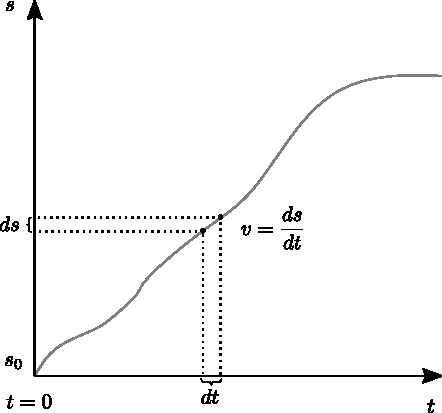
\includegraphics[width=\linewidth]{figures/stodutimagraf-orsmaed.pdf}
    \caption{Hraðinn er skilgreindur sem hallatalan í sérhverjum punkti á stöðu-tíma grafi.}
    \label{subfig:st-hradi}
\end{subfigure}
\caption{Með því að stöðugt minnka tímabilið þá fæst nákvæmara mat á punkthraða hlutarins.}
\end{figure}

\begin{tcolorbox}
\begin{definition}
Við skilgreinum \textbf{hraða} hlutar sem hallatölu snertils við stöðu-tímagrafið, þ.e.~
\begin{align*}
    v = \frac{ds}{dt}.
\end{align*}
\end{definition}
\end{tcolorbox}
\begin{tcolorbox}
\begin{definition}
Við skilgreinum \textbf{hröðun} hlutar sem hallatölu snertils við hraða-tímagrafið, þ.e.~
\begin{align*}
    a = \frac{dv}{dt}.
\end{align*}
\end{definition}
\end{tcolorbox}

\begin{figure}[H]
    \centering
\begin{subfigure}[h]{.4\textwidth}
    \centering
    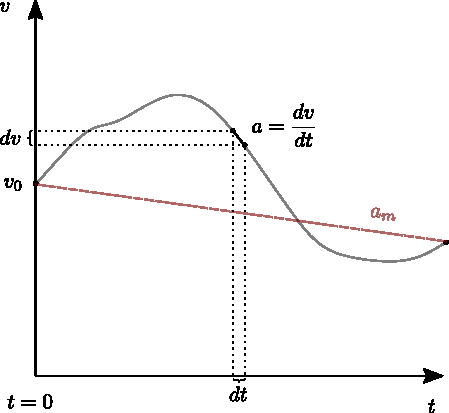
\includegraphics[width=\linewidth]{figures/hradatimagraf-hallatala.pdf}
    \caption{Á þessu hraða-tíma grafi sést bæði augnablikshröðunin $a$ og meðalhröðunin $a_m$.}
    \label{fig:vt-hradi}
\end{subfigure}
\hfill
\begin{subfigure}[h]{.4\textwidth}
    \centering
    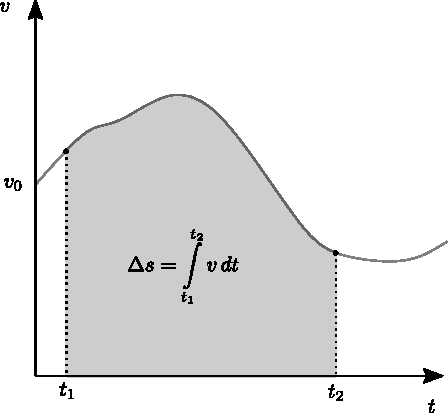
\includegraphics[width=\linewidth]{figures/hradatimagraf-flatarmalid.pdf}
    \caption{Flatarmálið undir hraða-tíma ferlinum jafngildir breytingu í stöðu hlutarins.}
    \label{fig:vt-tegur}
\end{subfigure}
\caption{Vinstri: Augnablikshröðun/meðalhröðun. Hægri: Samsvörun flatarmáls undir ferli við færslu.}
\end{figure}

\begin{tcolorbox}
\begin{theorem} \label{law:flatarmal}
Flatarmálið undir ferli hraða-tíma grafsins jafngildir færslunni. 
\end{theorem}
\end{tcolorbox}

\newpage

\begin{comment}
Við skulum loksins skýra nánar tengslin milli flatarmálsins undir ferlinum á hraða-tíma grafinu og stöðubreytingarinnar sem var ýjað að á mynd \ref{fig:vt-tegur}. Ef hraði hlutarins er jafn þá vitum við að $v_m = \frac{\Delta s}{\Delta t}$. En það er jafngilt því að $\Delta s = v_m \Delta t = v_m t$ með því að margfalda í gegn með $\Delta t$. En ef við skiptum up tímabilinu $t_1$ til $t_2$ í örlítil bil hvert með lengd $dt$ þá er það góð nálgun að á hverju þessara bila þá sé hraðinn fastur $v = \frac{ds}{dt}$. En þá gildir á þeim bilum einmitt að $ds = v dt$. Með því að leggja saman öll þessi gildi frá $t_1$ til $t_2$ (við notum ritháttinn $\int$ til að tákna þessa summu) fæst flatarmálið undir ferlinum milli $t_1$ og $t_2$.
\end{comment}


\section{Usain Bolt}

Þið kannist eflaust við það að Usain Bolt sé fljótasti maður heims. Til þess að skýra stöðu-tíma og hraða-tíma gröfin nánar þá má sjá gögn sem lýsa hlaupi hans á Ólympíuleikunum í Beijing árið 2008 hér fyrir neðan. Í myndbandsupptökum af hlaupinu þá sést hvernig Usain Bolt hægir á sér síðustu \SI{20}{m} hlaupsins. Það sést einnig greinilega á hraða-tíma grafinu hér fyrir neðan. Margir hafa velt fyrir sér hversu hratt hann hefði getað hlaupið ef hann hefði ekki hægt á sér síðustu metrana í því hlaupi.


\begin{comment}
\begin{figure}[H]
    \centering
    \gnuplotloadfile[terminal=epslatex, terminaloptions=color]{usain.gnu}
    \caption{þetta er graf af stöðu}
    \label{fig:my_label}
\end{figure}

\begin{figure}[H]
    \centering
    \gnuplotloadfile[terminal=epslatex, terminaloptions=color]{usain-speed.gnu}
    \caption{þetta er graf af hraða}
    \label{fig:lala}
\end{figure}
\end{comment}

\begin{table}[H]
\begin{minipage}[b]{0.38\linewidth}
\centering
\begin{tabular}{|c|c|}
\hline
\textbf{Vegalengd} [$\si{m}$] & \textbf{Tími} [$\si{s}$]\\
\hline
$5.0 \pm 0.5$ & $1.10 \pm 0.01$  \\
$10.0 \pm 0.5$ & $1.85 \pm 0.01$  \\
$20.0 \pm 0.5$ & $2.87 \pm 0.01$  \\
$34.0 \pm 0.4$ & $4.00 \pm 0.01$   \\
$41.3 \pm 0.5$ & $4.50 \pm 0.01$  \\
$52.1 \pm 0.5$ & $5.40 \pm 0.01$  \\
$55.9 \pm 0.5$ & $5.80 \pm 0.01$    \\
$61.5 \pm 0.5$ & $6.20 \pm 0.01$  \\
$64.8 \pm 0.4$ & $6.50 \pm 0.01$   \\
$69.6 \pm 0.2$ & $6.90 \pm 0.01$   \\
$73.3 \pm 0.2$ & $7.30 \pm 0.01$ \\
$81.7 \pm 0.2$ & $8.00 \pm 0.01$   \\
$85.6 \pm 0.2$ & $8.30 \pm 0.01$   \\
$89.2 \pm 0.2$ & $8.60 \pm 0.01$ \\
$91.3 \pm 0.2$ & $8.80 \pm 0.01$ \\
$98.6 \pm 0.2$ & $9.40 \pm 0.01$ \\
$100.0 \pm 0.1$ & $9.69 \pm 0.01$ \\
\hline
\end{tabular}
\label{tafla:usain1}
\caption{Tafla með mælingum Bolts.}
\end{minipage}\hfill
\begin{minipage}[b]{0.6\linewidth}
\centering
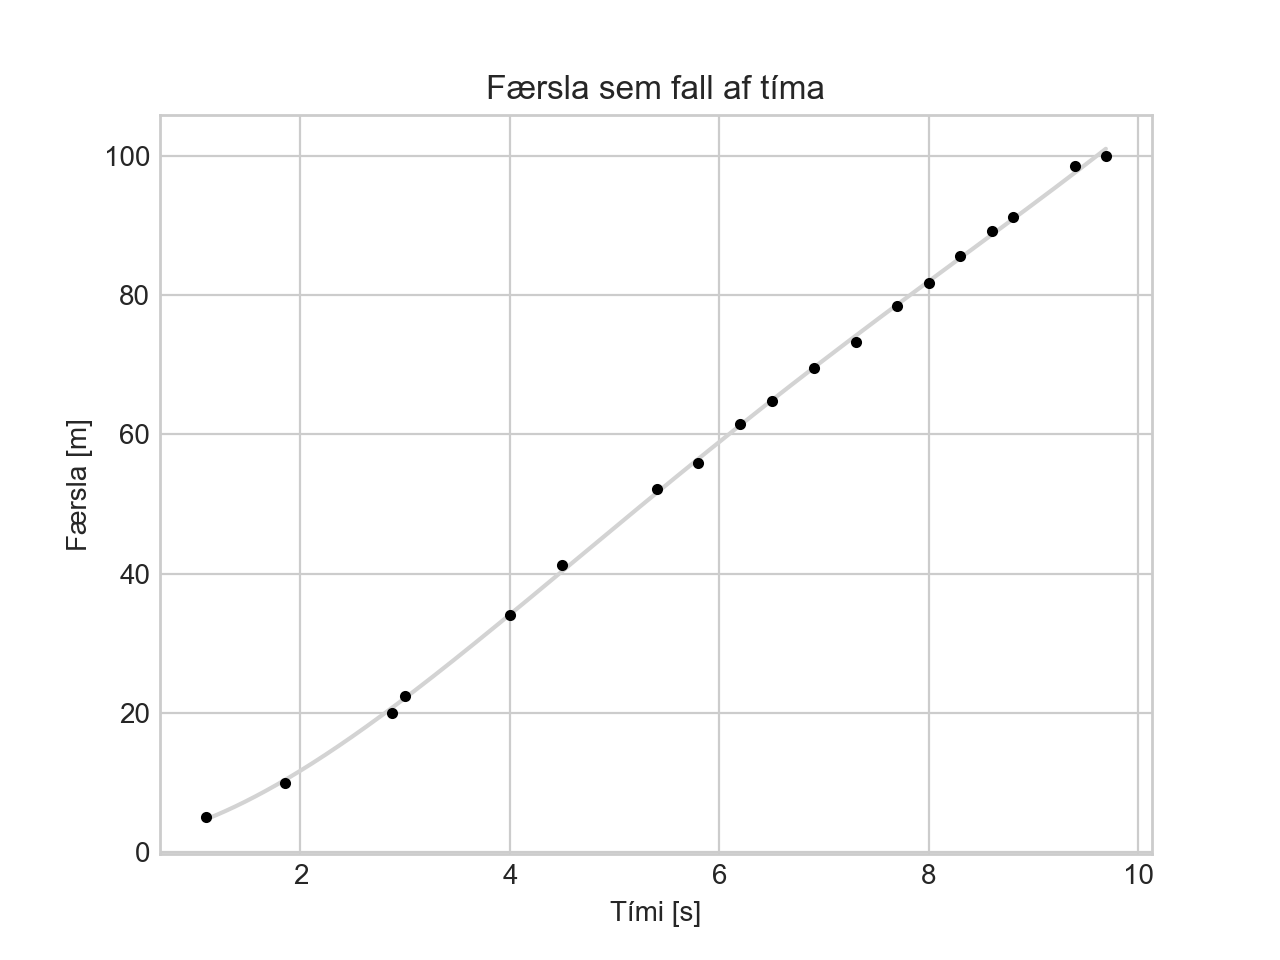
\includegraphics[scale = 0.6]{images/plot_1.png}
\caption{Graf sem sýnir stöðu Bolts sem fall af tíma.}
\label{fig:bolt1}
\end{minipage}
\end{table}


\begin{table}[H]
\begin{minipage}[c]{0.38\linewidth}
\centering
\begin{tabular}{|c|c|}
\hline
\textbf{Meðalhraði} [$\si{m/s}$] & \textbf{Tími} [$\si{s}$]\\
\hline
$4.54$ & $1.10$  \\
$5.40$ & $1.85$  \\
$10.0$ & $3.78$  \\
$11.5$ & $4.65$   \\
$11.8$ & $5.50$   \\
$12.2$ & $6.32$  \\
$12.2$ & $7.14$  \\
$12.2$ & $7.96$    \\
$12.0$ & $8.79$  \\
$11.1$ & $9.69$   \\
\hline
\end{tabular}
\label{tafla:usain2}
\caption{Mælingar á meðalhraða Bolts.}
\end{minipage}\hfill
\begin{minipage}[c]{0.6\linewidth}
\centering
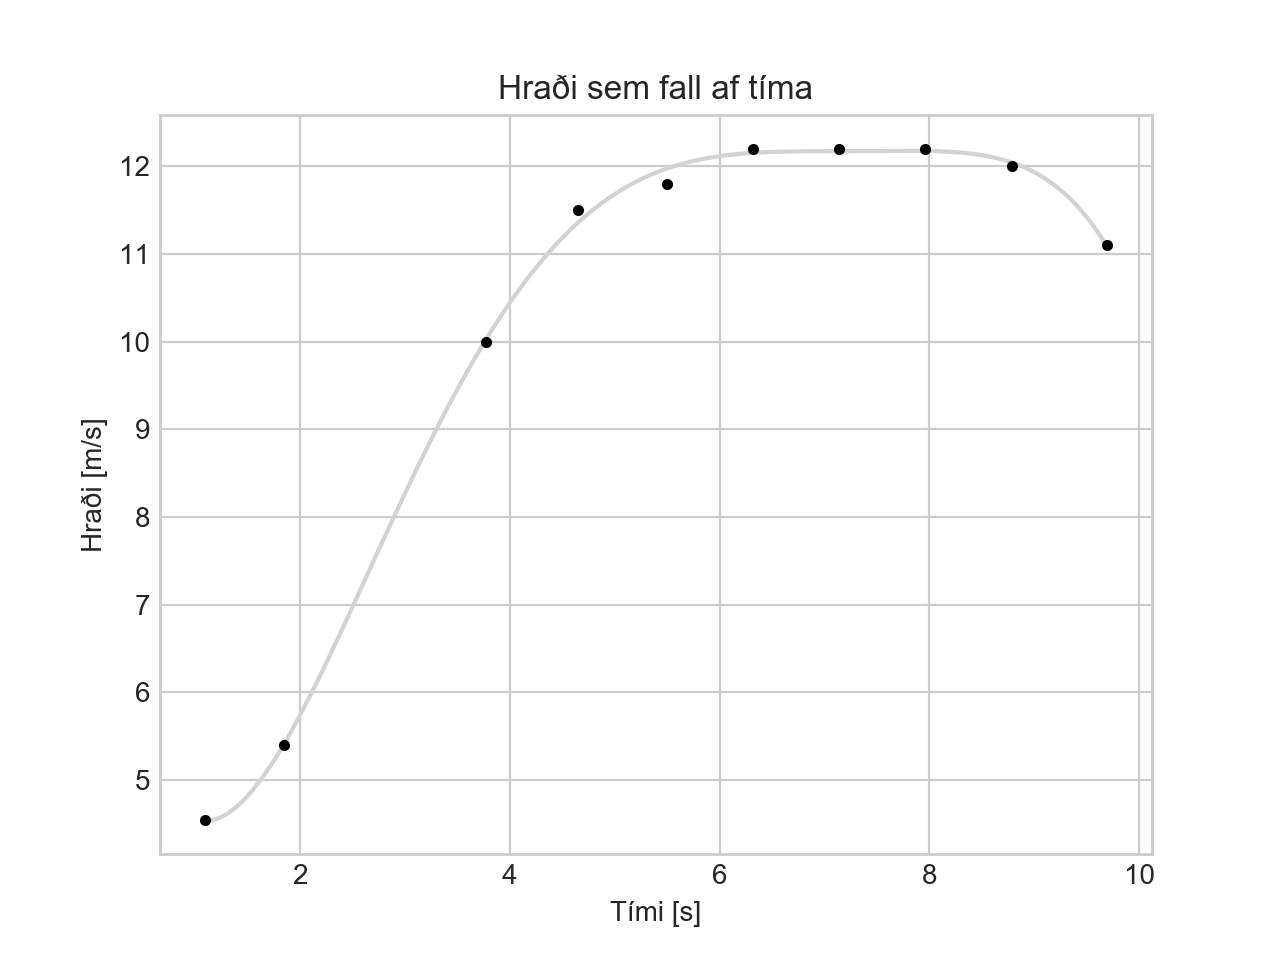
\includegraphics[scale = 0.6]{images/plot_2.png}
\caption{Graf sem sýnir meðalhraða Bolts sem fall af tíma.}
\label{fig:bolt2}
\end{minipage}
\end{table}

\newpage

\section{Föst hröðun og stöðujöfnurnar}

Við skulum núna skoða sértilfellið þegar hröðun hlutarins, $a$, er föst. Þið gætuð haldið að það væri afskaplega óáhugavert tilvik, en það er afskaplega mikilvægt. Til dæmis er þyngdarhröðun jarðar, $g = \SI{9.82}{m/s^2}$, föst. Helsti kosturinn við að skoða fasta hröðun er að það einfaldar lögun hraða-tíma grafsins afskaplega mikið og það samanstendur aðeins af beinum línum (sem þýðir að það er auðvelt að reikna flatarmálið undir ferlinum).

\begin{figure}[H]
    \centering
\begin{subfigure}[h]{.4\textwidth}
    \centering
    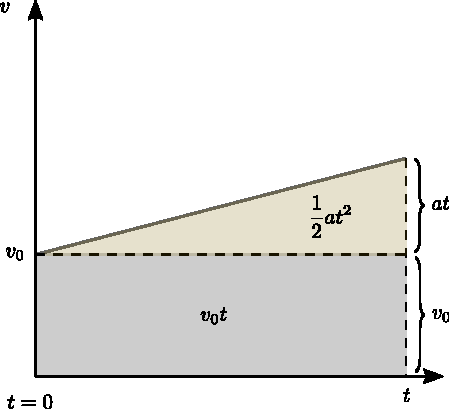
\includegraphics[width=\linewidth]{figures/hradatimagraf-sonnun.pdf}
    \caption{Hraða-tíma graf hlutar sem ferðast með fastri hröðun $a$.}
    \label{fig:fast-hrodun}
\end{subfigure}
\hfill
\begin{subfigure}[h]{.4\textwidth}
    \centering
    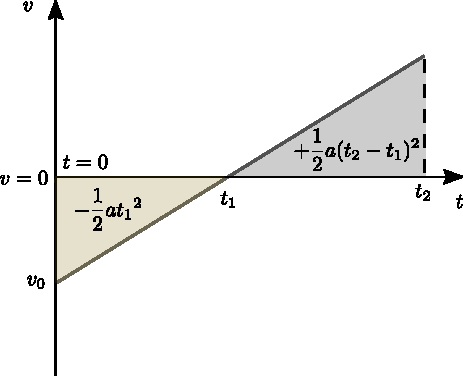
\includegraphics[width=\linewidth]{figures/hradatimagraf-neikvaett.pdf}
    \caption{Hraða-tíma graf með neikvæðan upphafshraða $v_0$ og fasta hröðun $a$.}
    \label{fig:neikvaett-hrodun}
\end{subfigure}
\caption{Hraða-tíma gröf með fastri hröðun $a$.}
\end{figure}


\begin{tcolorbox}
\begin{theorem}
Lítum á hlut sem er upphaflega staddur í $s_0$ og hefur upphafshraða $v_0$. Gerum ráð fyrir að hluturinn verði fyrir fastri hröðun $a$. Látum $s$ tákna stöðu hlutarins og $v$ tákna hraða hlutarins eftir tímann $t$. Þá gilda stöðujöfnurnar:

\begin{enumerate}[label = \textbf{(\roman*)}]
    \item $v = v_0 + at$.

    \item $s = s_0 + v_0 t + \frac{1}{2}at^2$.
    
    \item $2a \Delta s = v^2 - v_0^2$.
\end{enumerate}
\end{theorem}
\end{tcolorbox}


\textbf{Útleiðsla:}
Með mynd \ref{fig:fast-hrodun} í huga þá athugum við að:
\begin{enumerate}[label = \textbf{(\roman*)}]
    \item Þar sem hröðunin er föst er hún jöfn meðalhröðuninni, þ.e.a.s. $a = \frac{\Delta v}{\Delta t}$ en það þýðir einmitt að $\Delta v = a \Delta t$ sem er það sama og að segja að $v - v_0 = at$, þ.e. $v = v_0 + at$.
    
    \item Með lögmál \ref{law:flatarmal} í huga þá hefjumst við handa við að reikna flatarmálið undir hraða-tíma grafinu. Við tökum fyrst eftir ferhyrningnum á mynd \ref{fig:fast-hrodun} sem hefur hæðina $v_0$ og breiddina $t$ og hefur því flatarmálið $v_0 t$. Hinsvegar tökum við eftir þríhyrningnum á mynd \ref{fig:fast-hrodun} sem hefur hæðina $at$ samkvæmt stöðujöfnu (i) hér á undan og breiddinna $t$. En þar með er flatarmál þríhyrningsins gefið með $\frac{1}{2} (at) t = \frac{1}{2}at
   ^2$. Heildarflatarmálið er því einmitt:
   \begin{align*}
       \Delta s = v_0 t + \frac{1}{2}at^2.
   \end{align*}
   
   \item Samkvæmt stöðujöfnu (i) höfum við að $t = \frac{v-v_0}{a}$. Við stingum því inn í stöðujöfnu (ii) og fáum:
   \begin{align*}
       \Delta s = v_0 t + \frac{1}{2}a t^2 = v_0 \left( \frac{v-v_0}{a} \right) + \frac{1}{2}a \left( \frac{v-v_0}{a} \right)^2 = \frac{v v_0}{a} -\frac{{v_0}^2}{a} + \frac{v^2}{2a} - \frac{v v_0}{a} + \frac{{v_0}^2}{2a} = \frac{v^2-{v_0}^2}{2a}. 
   \end{align*}
   Með því að margfalda í gegn með $2a$ fáum við einmitt að $2a \Delta s = v^2 - {v_0}^2$. \qed
\end{enumerate}

\begin{comment}
\begin{proof}
\textbf{(Ekki til prófs)}. Til þess að sanna þessar niðurstöður fyllilega þurfum við að beita stærðfræðigreiningu. Þar sem að $a = \text{fasti}$ höfum við með því að aðskilja breytistærðir og tegra:
\begin{align*}
    a = \frac{dv}{dt} \implies \int_{v_0}^{v} dv = \int_{0}^{t} a dt \implies v-v_0 = at
\end{align*}
Sem við getum umritað yfir á sama form og í (ii) til að fá:
\begin{align*}
    v = v_0 + at.
\end{align*}
Með því að tegra jöfnuna aftur fáum við að:
\begin{align*}
    v = \frac{ds}{dt} \implies  \int_{s_0}^{s} ds = \int_0^t v dt \implies   s-s_0 = \int_0^t \left( v_0 + at \right)dt = v_0 t + \frac{1}{2} a t^2.
\end{align*}
Sem við getum umritað yfir á sama form og í (i) til að fá:
\begin{align*}
    s = s_0 + v_0 t + \frac{1}{2}at^2.
\end{align*}
Síðasta jafnan þarf örlítið trikk, sem er oftast nefnt keðjureglan. Við athugum að:
\begin{align*}
    a = \frac{dv}{dt} = \frac{dv}{ds}\frac{ds}{dt} = \frac{dv}{ds} v
\end{align*}
þar sem að við höfum lengt brotið með $ds$ í einhverjum skilningi til að gera stærðfræðina auðveldari. Nú þegar við tegrum fáum við að:
\begin{align*}
    a = \frac{dv}{ds}v \implies \int_{s_0}^s a ds = \int_{v_0}^{v} v dv \implies a (s-s_0) = \frac{1}{2}\left( v^2 - v_0^2\right)
\end{align*}
En það gefur okkur einmitt að:
\begin{align*}
    2a\Delta s = v^2 - v_0^2
\end{align*}
\end{proof}
\end{comment}

\newpage

\section{Dæmi}

\begin{enumerate}[label = \textbf{Dæmi \thechapter.\arabic*.}]

\subsection*{Hraði}

\item Ökumenn þurfa að gæta að þriggja sekúndna reglunni til að tryggja nægilegt bil á milli bíla í umferðinni. Bíll keyrir á \SI{90}{km/klst}. Hversu langa vegalengd ferðast hann á þremur sekúndum?

\item Vegalengdin frá Reykjavík til Leifsstöðvar er rúmir $\SI{50}{km}$. Anna og Baldur eru í kapphlaupi. Anna keyrir á löglegum hámarkshraða, $\SI{90}{km/klst}$ á meðan Baldur keyrir ólöglega á $\SI{100}{km/klst}$. Ef Anna og Baldur leggja af stað á sama tíma frá Reykjavík, hversu miklum tíma munar á því hvenær þau koma fram á áfangastaðinn?

\item Heiðlóan er farfugl sem kemur til Íslands í lok mars eftir vetrarsetu í Bretlandseyjum. Hún getur flogið með allt að $\SI{80}{km/klst}$ meðalhraða. Ef vegalengdin frá Bretlandseyjum til Íslands er rúmir $\SI{1500}{km}$, hversu langan tíma tekur það heiðlóuna að fljúga til Íslands?

\item Meðalfjarlægðin milli jarðarinnar og sólarinnar er $\SI{1}{AU} = \SI{1.50e11}{m}$. Tíminn sem það tekur jörðina að fara einn hring í kringum sólina er eitt ár. Hver er meðalhraði jarðarinnar á braut sinni um sólina?

\item Lilja sér blossa frá flugeldi og heyrir hvellinn \SI{3.00}{s} síðar. Hve langt frá flugeldinum stendur Jóhanna ef hljóðhraðinn er $v_{\text{hljóð}} = \SI{343}{m/s}$?

\item Jörmunrekur er mættur í Keiluhöllina í Egilshöll. Keilubrautirnar þar eru \SI{18.3}{m} langar. Jörmunrekur hendir kúlunni sinni þannig að hún rennur eftir brautinni með föstum hraða. Hann heyrir kúluna skella á keilunum \SI{2.80}{s} eftir að hann kastaði kúlunni. Hver var hraði keilukúlunnar?

\item Tvær járnbrautalestir nálgast óðfluga á sömu lestarteinunum. Báðar lestirnar eru að ferðast með jöfnum hraða, $\SI{155}{km/klst}$. Vegalengdin á milli lestanna er til að byrja með $\SI{8.5}{km}$. Hversu langur tími mun líða þar til að lestarnar skella saman?  

\begin{figure}[H]
    \centering
    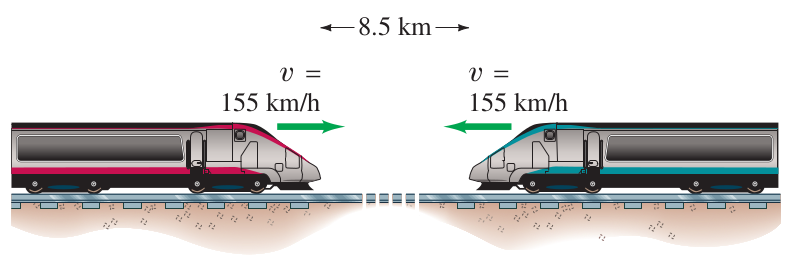
\includegraphics[scale = 0.25]{images/lestir.png}
    \caption{Mynd af lestunum tveim.}
    \label{fig:lestir}
\end{figure}

\item Bíll sem ferðast með jöfnum hraða $\SI{95}{km/klst}$ tekur fram úr flutningalest sem ferðast með jöfnum hraða \SI{75}{km/klst}. Flutningalestin er $\SI{1.30}{km}$ að lengd. 
\begin{enumerate}[label = \textbf{(\alph*)}]
    \item Hversu langan tíma tekur það bílinn að taka fram úr lestinni?
    
    \item Hversu langa vegalengd hefur bíllinn ferðast á þeim tíma?
\end{enumerate}

\begin{figure}[H]
    \centering
    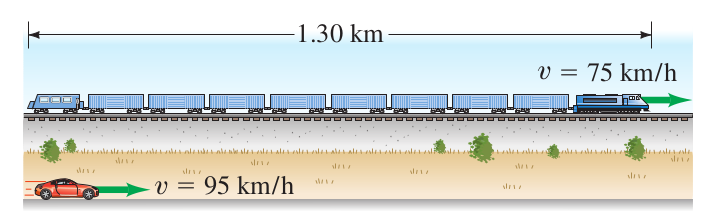
\includegraphics[scale = 0.35]{images/bill.png}
    \caption{Mynd af bílnum og lestinni.}
    \label{fig:framur}
\end{figure}

\subsection*{Hröðun}

\item Formúlubíll Lewis Hamiltons getur tekið af stað úr kyrrstöðu og náð \SI{200}{km/klst} á \SI{4.4}{s}.
\begin{enumerate}[label = \textbf{(\alph*)}]
    \item Hver er meðalhröðun bílsins á þeim tíma? 
    \item Metið vegalengdina sem hann ferðast á þeim tíma. 
\end{enumerate}


\item Bíll keyrir með \SI{50}{km/klst} hraða  þegar hann kemur inn í götu þar sem hámarkshraðinn er $\SI{30}{km/klst}$. Hann hemlar í \SI{3.6}{s} til að hægja á sér. Hver var meðalhröðun bílsins á þeim tíma?

\item Usain Bolt tekur af stað úr kyrrstöðu og nær \SI{12.2}{m/s} hraða á \SI{5.68}{s}. Hver var meðalhröðun Bolts?

\subsection*{Stöðujöfnurnar}

\item Bíll breytir hraða sínum úr $\SI{14}{m/s}$ í $\SI{21}{m/s}$ á $\SI{6.0}{s}$. Hver var meðalhröðun bílsins á þeim tíma? Hversu langa vegalengd ferðaðist bíllinn á þeim tíma?

\item Einkaflugvél Jeff Bezos þarf að ná $\SI{35}{m/s}$ hraða til að geta tekið á loft. Hversu löng þarf flugbrautin að vera ef meðalhröðun flugvélarinnar er $\SI{3.0}{m/s^2}$?

\item Þyngdarhröðun jarðar er $g = \SI{9.82}{m/s^2}$. Köttur nokkur dettur fram af svölum á þriðju hæð og lendir á jörðinni $\SI{1.1}{s}$ síðar. Kötturinn lifir af fallið sem betur fer! Úr hversu mikilli hæð féll kötturinn?

\item Hæsta bygging í heimi er Burj Khalifa turnin sem er staðsettur í Dubai í Sameinuðu arabísku furstadæmunum. Hann er $\SI{830}{m}$ á hæð. Hugsum okkur manneskju sem fellur fram af toppi turnsins. Hversu langur tími líður þar til að manneskjan lendir á jörðinni? Hver væri hraði manneskjunnar rétt áður en hún skellur á jörðinni og upplifir voveiflegan dauðdaga sinn?

\item Í ökuskóla 3 er fólk stundum fengið til þess að nauðhemla á \SI{80}{km/klst} hraða.
Mesta hemlunarhröðun sem að ökumaður getur haldið stjórn á bílnum við er um það bil \SI{6.0}{m/s^2}. Hver er minnsta vegalengdin sem bílinn ferðast þar til ökumaðurinn nær að stöðva bílinn án þess þó að missa stjórn á honum?


\item Sigga litla er bráðgáfuð og ætlar að mæla dýptina á brunninum í sveitinni sinni með sniðugri aðferð. Hún sleppir stein ofan í brunninn og heyrir hann lenda í vatninu eftir $\SI{1.3}{s}$. Hversu djúpur er brunnurinn?


\item Sigga og Magga eru að taka þátt í Maraþonhlaupi. Þegar Sigga er $\SI{22}{m}$ frá endamarkinu er hraði hennar $\SI{5.0}{m/s}$. Magga er $\SI{5.0}{m}$ fyrir aftan Siggu og hleypur með hraða $\SI{4.0}{m/s}$. Sigga telur sigurinn vera í höfn og byrjar að hægja á sér með fastri hröðun $-\SI{0.40}{m/s^2}$ þar til hún kemur í mark. Magga sér sér leik á borði og ákveður að gefa í síðustu metrana. Hver þarf hröðun Möggu að vera restina af hlaupinu til þess að þær komi jafnar 
í mark?

\begin{figure}[H]
    \centering
    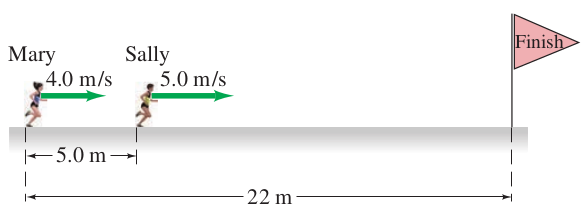
\includegraphics[scale = 0.35]{images/kapphlaup.png}
    \caption{Síðustu metrarnir í maraþonhlaupinu.}
    \label{fig:kapphlaup}
\end{figure}

\item Lalli leynilögreglumaður ferðast í bíl með upphafshraða \SI{95}{km/klst} þegar ökuníðingur nokkur tekur fram úr honum á \SI{135}{km/klst}. Nákvæmlega $\SI{1.00}{s}$ eftir að ökuníðingurinn tekur fram úr Lalla byrjar Lalli að gefa í og eykur hraðann sinn með jafnri hröðun $a = \SI{2.60}{m/s^2}$. Hversu langur tími líður þar til að Lalli nær ökuníðingnum ef ökuníðingurinn heldur jöfnum hraða? 

\subsection*{Stöðu-tíma og hraða-tíma gröf}

\begin{minipage}{\linewidth}

\begin{wrapfigure}{r}{2.6in}
\vspace{-1cm}
\centering
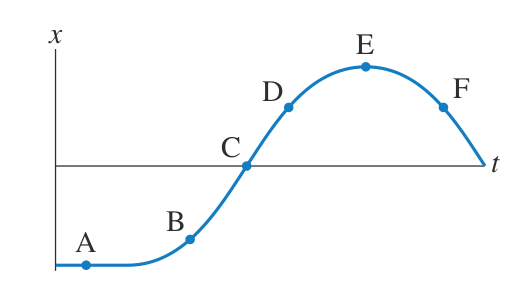
\includegraphics[width=2.5in]{images/stada.png}
\caption{Staða, $x$, sem fall af tíma, $t$.}
\label{fig:stodutima}
\end{wrapfigure}

\item Lítum á stöðu-tíma grafið hér fyrir neðan á mynd \ref{fig:stodutima}. Í hvaða punktum
\begin{enumerate}[label = \textbf{(\alph*)}]
    \item Var hraði hlutarins mestur?
    \item Var hluturinn að ferðast til vinstri?
    \item Var hluturinn að auka hraða sinn?
    \item Var hluturinn að snúa við?
\end{enumerate}

\end{minipage}

\vspace{1cm}

\begin{minipage}{\linewidth}

\begin{wrapfigure}{r}{2.6in}
\vspace{-1cm}
\centering
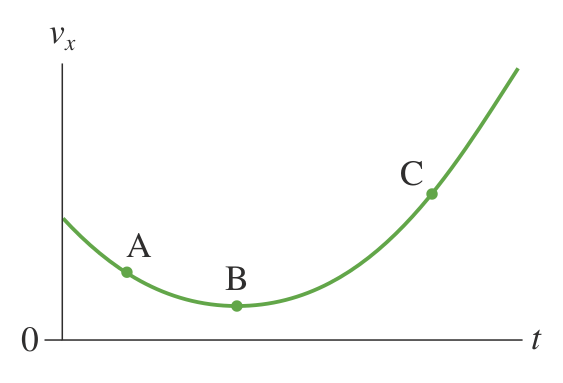
\includegraphics[width=2.5in]{images/hradatima.png}
\caption{Hraði, $v_x$, sem fall af tíma, $t$.}
\label{fig:hradatima}


\end{wrapfigure}

\item Lítum á hraða-tíma grafið hér fyrir neðan á mynd \ref{fig:hradatima}. Í hvaða punktum
\begin{enumerate}[label = \textbf{(\alph*)}]
    \item Er hluturinn að auka hraða sinn?
    \item Er hluturinn að hægja á sér?
    \item Er hluturinn að ferðast til vinstri?
    \item Er hluturinn að ferðast til hægri?
\end{enumerate}

\end{minipage}

\vspace{1cm}

\begin{minipage}{\linewidth}

\begin{wrapfigure}{r}{2.6in}
\vspace{-0.5cm}
\centering
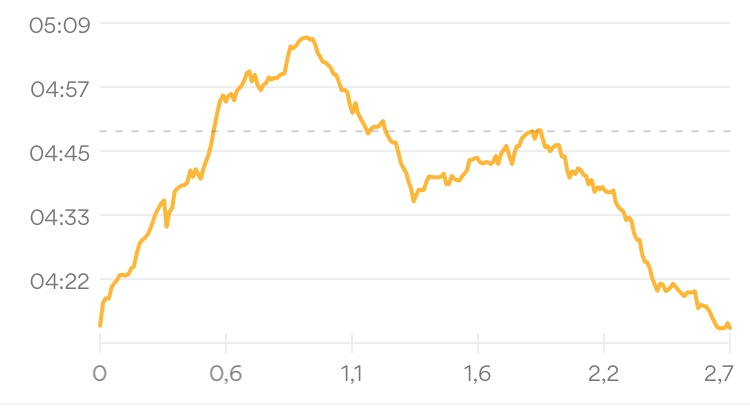
\includegraphics[width=2.5in]{images/hlaupa.jpg}
    \caption{Hraða-stöðu graf hlauparans.}
    \label{fig:myRunkeeper}

\end{wrapfigure}

\item Lítum á eftirfarandi graf sem fengið er úr hlaupaforritinu Runkeeper. Á lárétta ás grafsins má greina \si{km} fjölda hlaupsins. Á lóðrétta ásnum má greina hraða hlauparans í einungunum sem samsvara því hversu fljótur hann væri að hlaupa \SI{1}{km} ef hann héldi þeim hraða. Gráa línan táknar meðalhraða hlauparans.
\begin{enumerate}[label = \textbf{(\alph*)}]
    \item Hver var meðalhraði hlauparans í $\si{m/s}$?
    \item Hver var mesti hraði hlauparans í hlaupinu?
    \item Hver var minnsti hraði hlauparans í hlaupinu?
\end{enumerate}

\end{minipage}

\vspace{1cm}

\begin{minipage}{\linewidth}

\begin{wrapfigure}{r}{2.6in}
\centering
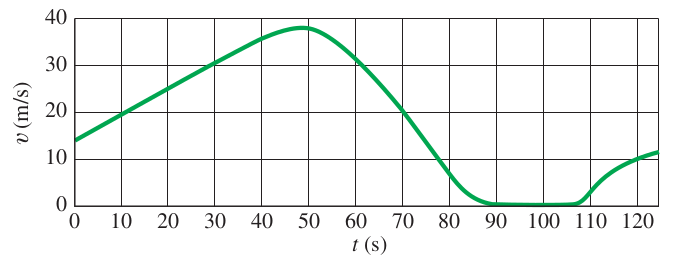
\includegraphics[width=2.5in]{images/lest-graf.png}
    \caption{Hraða-tíma graf lestarinnar.}
    \label{fig:lest-hradi}

\end{wrapfigure}

\item Lítum á hraða-tíma grafið á mynd \ref{fig:lest-hradi} sem sýnir hraða járnbrautalestar sem fall af tíma, $t$.
\begin{enumerate}[label = \textbf{(\alph*)}]
    \item Á hvaða tíma var hraði lestarinnar mestur?
    \item Ferðaðist lestin einhvern tímann með jöfnum hraða?
    \item Ferðaðist lestin einhvern tímann með jafnri hröðun?
    \item Við hvaða tíma var hröðun lestarinnar mest?
    \item Hversu langa vegalengd ferðaðist lestin?
\end{enumerate}

\end{minipage}


\newpage

\subsection*{Gömul prófdæmi}

\item Ef bolta væri sleppt þannig að hann myndi falla niður að eilífu með fastri hröðun, $g = \SI{9.82}{m/s^2}$ þá myndi hann á einhverjum tímapunkti ná ljóshraða, $c = \SI{3.00e8}{m/s}$.
\begin{enumerate}[label = \textbf{(\alph*)}]
\item Hversu margar sekúndur myndi það taka boltann að ná ljóshraða?
\item Hversu marga daga myndi það taka boltann að ná ljóshraða?
\item Hversu langa vegalengd hefði boltinn fallið þá?
\end{enumerate}

\item Sigurlaug er að bruna niður Kringlumýrarbrautina á $\SI{100}{km/klst}$ þegar hún sér gamla konu á veginum $\SI{50.0}{m}$ fyrir framan sig. Hún nauðhemlar með fastri hröðun $a = -\SI{7.80}{m/s^2}$ í von um að ná að bjarga gömlu konunni. Hversu langt fer Sigurlaug áður en hún nær að stöðva bílinn? Nær hún að bjarga gömlu konunni?

\item Vilbert vörubílstjóri keyrir á hraðanum $\SI{16}{m/s}$ niður Sviðholtsvör. Skyndilega verður hann var við Leif litla sem er að byrja að fara yfir gangbraut á hlaupahjólinu sínu með hraðanum $\SI{1.6}{m/s}$. Vilbert er í $\SI{20}{m}$ fjarlægð þegar hann byrjar að hemla með hröðuninni $\SI{-6.2}{m/s^2}$ í von um að Leifur nái að forða sér undan vörubílnum í tæka tíð. Breidd vörubílsins er $\SI{2.5}{m}$. Nær Leifur litli að forða sér undan vörubílnum ef hann heldur sama hraða?

\item Geimflaug er skotið upp í loftið. Þegar geimflaugin hefur náð hraðanum $\SI{200}{m/s}$ er það í $\SI{5.0}{km}$ hæð. Þá áttar Neil Armstrong sig á því að hann gleymdi geimbúningnum sínum heima. Hann stekkur því úr geimflauginni til þess að sækja búninginn. Honum til mikillar undrunar byrjar hann ekki að detta niður alveg strax. Hann fer fyrst upp með sama hraða og geimflaugin svo hægist á honum smátt og smátt þar til hann stoppar um stund og fellur svo til jarðar með þyngdarhröðuninni $g$.
\begin{enumerate}[label = \textbf{(\alph*)}]
\item Finnið tímann $t$ sem líður áður en hann byrjar að detta niður.
\item Finnið $s_{\text{max}} > \SI{5000}{m}$ sem lýsir hversu hátt hann kemst áður en hann byrjar að detta.
\end{enumerate}

\begin{minipage}{\linewidth}

\begin{wrapfigure}{r}{0.2in}

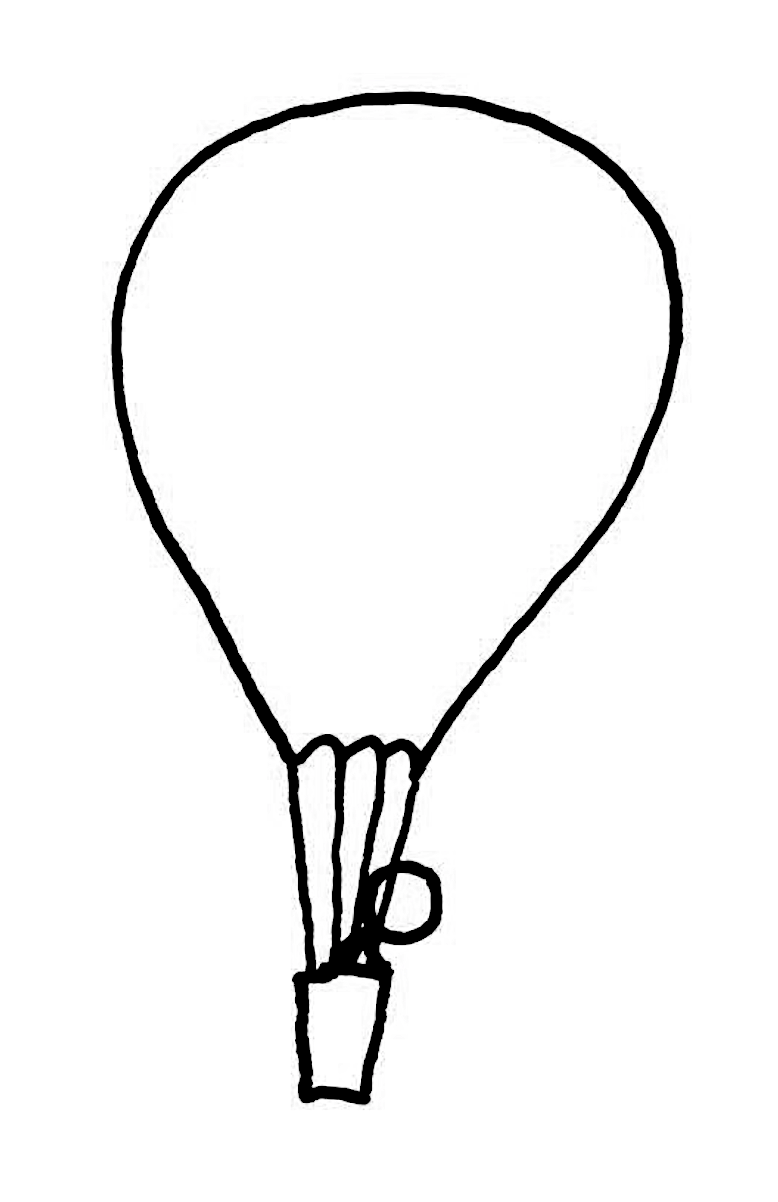
\includegraphics[width=1 in]{images/loftbelgur.png}

\end{wrapfigure}

\item
Lambert loftbelgskóngur hefur gaman að því að fljúga um frönsku háloftin. Hann tekur sér matarpásu í $\SI{800}{m}$ hæð. Skyndilega rekur fugl gogginn í loftbelginn (sem er kyrr) og gerir gat á hann. Loftbelgurinn byrjar þá að hrapa með lóðréttri hröðun $\SI{2.4}{m/s^2}$. Hunsið loftmótsstöðu.
\begin{enumerate}[label = \textbf{(\alph*)}]
\item Hversu langur tími mun líða þar til að loftbelgurinn skellur á jörðinni?
\item
Lambert nær hinsvegar að loka fyrir gatið með baguette úr matarkörfunni sinni eftir að hafa hrapað í $\SI{10}{s}$. Þá er hann í $\SI{680}{m}$ hæð og hefur hraðann $\SI{24}{m/s}$ niður á við. Eftir að gatinu er lokað fær loftbelgurinn hröðun $\SI{1.3}{m/s^2}$ upp á við. Hver verður minnsta hæð loftbelgsins yfir jörðu?
\end{enumerate}
\end{minipage}



\item Herdís situr við glugga uppi á $3.$ hæð. Hún er að leika sér með litla málmkúlu. Hún hendir kúlunni upp í loft með hraðanum $\SI{2.0}{m/s}$ og grípur hana aftur.
\begin{enumerate}[label = \textbf{(\alph*)}]
    \item Hversu hátt upp fer kúlan?
    \item Nú tapar Herdís athyglinni eitt augnablik og missir af kúlunni svo hún fellur alla leið niður á stétt. Kúlan lendir á stéttinni $\SI{1.4}{s}$ sekúndum eftir að Herdís sleppir henni. Hversu hátt uppi er glugginn?
\end{enumerate}

\item Lítum á hlut sem ferðast með fastri hröðun $a$. Látum upphafshraða hlutarins vera gefinn með $v_0$ og látum lokahraða hans vera gefinn með $v$. Sýnið með skilgreiningu á meðalhraða, $v_m$, að $v_m = \frac{v + v_0}{2}$.

\item Vagn með massa $m = \SI{0,65}{kg}$ stendur á braut sem hallar um horn $\theta$ miðað við lárétt. Hann byrjar að renna niður \SI{2,4}{m} langa brautina úr kyrrstöðu í hæðinni $\SI{0,63}{m}$. Tíminn sem þetta tekur mælist $\SI{1,45}{s}$.
    \begin{enumerate}[label = \textbf{(\alph*)}]
        \item Finnið meðalhraða vagnsins, $v_m$, á leiðinni niður.
        \item Finnið lokahraða vagnsins á leið sinni niður brautina.
    \end{enumerate}


\newpage



\section*{Dæmin sem 5.Y samdi}

\item \textbf{(Elísa, Eva og Hildur)} Lalli er í teygjustökki sem er $\SI{50}{m}$. Hann lætur sig falla beint niður með hröðun $g = \SI{9.82}{m/s^2}$.
\begin{enumerate}[label = \textbf{(\alph*)}]
    \item Hver er hraði Lalla rétt áður en hann er kominn niður?
    \item Hvað tekur það langan tíma að komast niður?
\end{enumerate}

\item \textbf{(Aðalheiður og Davíð Þór)} Eiffel turninn er $\SI{324}{m}$ á hæð. Ef þú lætur bolta detta af toppnum, hver er hraði boltans rétt áður en hann skellur á jörðina?

\item \textbf{(Egill og Davíð Freyr)} Davíð og Egill eru í listflugi í \SI{12.8}{km} hæð en allt í einu dettur Davíð úr vélinni. Að $\SI{5}{s}$ liðnum fattar Egill að Davíð datt og þá steypir hann vélinni beint niður með hraða $\SI{52}{m/s}$ (og með sömu hröðun og Davíð). Nær Egill að grípa Davíð áður enn hann verður að pönnuköku? Eftir hversu langan tíma ef svo er?

\item \textbf{(Kristján og Oddur)} Jörðin er hnöttótt. Það leggja tvær flugvélar af stað og eru í $\SI{36.3}{km}$ hæð. Flugvélar A og B fljúga af stað frá Ecuador og fljúga meðfram miðbaug jarðar austur. Jörðin snýst $\SI{1600}{km/klst}$. Flugvél A flýgur á $\SI{800}{km/klst}$ en flugvél B á $\SI{750}{km/klst}$.
\begin{enumerate}[label = \textbf{(\alph*)}]
    \item Eftir hve marga kílómetra hringar flugvél A flugvél B?
    \item Yfir hvaða lengdarbaug hringar flugvél A flugvél B?
\end{enumerate}

\section*{Dæmin sem 5.X samdi}

\item \textbf{(María, Ylja, Sandra og Ingibjörg)} Siggi litli er búinn að eyða allri ævi sinni í að grafa holu í gegnum jörðina. Gummi stóri stendur hinum megin á jörðinni og bíður eftir flöskuskeyti frá Sigga.
\begin{enumerate}[label = \textbf{(\alph*)}]
    \item Hversu hratt fer flöskuskeytið í gegnum jörðina miðað við að $g = \SI{9.82}{m/s^2}$
    
    \item Hvað er flöskuskeytið lengi á leiðinni til Gumma?
\end{enumerate}

\item \textbf{(Stefán, Benedikt, Einar Atli)} Stefán er að verða seinn á æfingu. Hann keyrir á $\SI{200}{km/klst}$. Hann þarf að keyra $\SI{366.3}{km}$ til að komast á lasertag æfingu. Þegar hann á $\SI{69}{km}$ eftir á áfangastað fattar hann að það er bara korter í æfinguna. Hvað þarf hröðunin að vera mikil til að hann nái æfingunni?

\item \textbf{(Stefán, Benedikt, Einar Atli)} Hversu margar pingpong kúlur kæmust fyrir inni í tunglinu.

\item \textbf{(Haraldur, Hjörtur, Ólafur)} Hjörtur byrjar með $\SI{2000}{m}$ forskot á Toyota Corola. Haraldur er á Golf R og þeir byrja á sama tíma. Haraldur kemst frá $\SI{0}{km/klst}$ upp í $\SI{240}{km/klst}$ á $\SI{8}{s}$. Hjörtur kemst frá $\SI{0}{km/klst}$ upp í $\SI{140}{km/klst}$ á $\SI{25}{s}$. Hversu lengi er Haraldur að ná Hirti á beinni braut.

\item \textbf{(Alex, Jovan og Bergur)} Hversu mörg súrefnisatóm eru í himinhvolfinu?

\item \textbf{(Gísli, Einar Skúli)} Hallgrímskirkja er mjög stór en þó ekki jafnstór og Esjan. Hversu mörg skákpeð kæmust inn í Esjuna ef hún væri hol að innan?

\end{enumerate}

\newpage